\chapter{Definici\'on del Problema}

\section{Información previa a considerar}

Para entrar de lleno en la tema, es necesario conocer de antemano varios aspectos básicos de la biología.

\subsection{Biomoléculas}

Cada vez que se habla de la biología, este concepto se relaciona directamente con la ciencia que estudia a los seres vivos. Ahora bien, las estructuras o compuestos que constituyen una parte esencial de los seres vivos son conocidas como \textbf{biomoléculas}. Estas biomoléculas están principalmente constituidas por elementos químicos como el carbono (C), hidrógeno (H), oxígeno (O), nitrógeno (N), fósforo (P) y azufre (S) \cite{biomolecula} y se pueden clasificar en biomoléculas inorgánicas, que se encuentran tanto en seres vivos como en los cuerpos inertes, no obstante son imprescindibles para la vida; y las biomoléculas orgánicas, que son sintetizadas por los seres vivos y tienen una estructura con base en carbono. Estas biomoléculas orgánicas se pueden separar en 4 grandes grupos:
\begin{enumerate}
\item Glúcidos (hidratos de carbono o carbohidratos): son la fuente de energía primaria que utilizan los seres vivos para realizar sus funciones vitales. Los ejemplos más conocidos son la glucosa, el almidón y el glucógeno.
\item Lípidos: conforman el principal almacén de energía de los animales y desempeñan funciones reguladores de enzimas y hormonas.
\item Ácidos nucleicos: El ácido desoxirribonucleico y el ácido ribonucleico, mayormente conocidos como ADN (DNA) y ARN (RNA y sus derivados) desarrollan posiblemente la función más importante para la vida: contener, de manera codificada, las instrucciones necesarias para el desarrollo y funcionamiento de la célula. El ADN tiene la capacidad de replicarse, transmitiendo así dichas instrucciones a las células hijas que heredarán la información.
\item Proteínas: poseen la mayor diversidad de funciones que realizan en los seres vivos; prácticamente todos los procesos biológicos dependen de su presencia y/o actividad. Son proteínas casi todas las enzimas, catalizadores de reacciones metabólicas, hemoglobina, anticuerpos, entre otros. Su unidad base es el {\it{aminoácido}}, por el cual se van formando los péptidos según la cantidad de unidades bases enlazadas.
\end{enumerate}

Dentro de estas biomoléculas, el análisis detallado de los carbohidratos y los lípidos depende en demasía de su estructura química (elementos químicos asociados y tipo de enlaces entre ellos), por lo mismo es una materia más ligada a los químicos (ver Figura 1.1). 

\begin{figure}[H] 

\begin{subfigure}{0.5\textwidth}
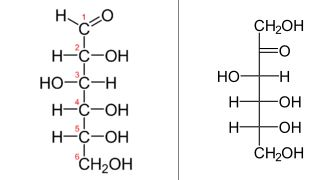
\includegraphics[width=0.9\linewidth, height=5cm]{./images/glucidoejemplos} 
\caption{Glúcidos (glucosa y fructosa)}
\label{fig:subim1}
\end{subfigure}
\begin{subfigure}{0.4\textwidth}
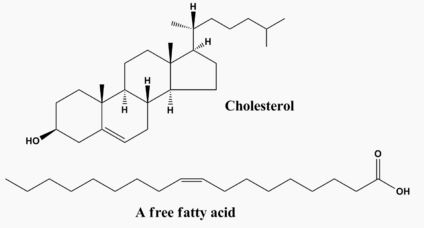
\includegraphics[width=1\linewidth, height=5cm]{./images/lipidosejemplos}
\caption{Lípidos (colesterol y un ácido graso)}
\label{fig:subim2}
\end{subfigure}
 
\caption{Estructura química de los carbohidratos y lípidos.}
\label{fig:image1}
\end{figure}

Sin embargo, el ADN y los polipéptidos poseen unidades base que pueden ser codificadas como letras, por consiguiente pueden ser secuenciados como {\it{cadenas de strings}} y en donde los avances computacionales y la evolución informática toman una importante relevancia (ver Figura 1.2).

\begin{figure}[H]

\begin{subfigure}{0.5\textwidth}
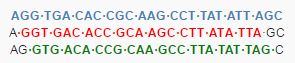
\includegraphics[width=1\linewidth, height=2cm]{./images/adnejemplo}
\caption{Cadena de ADN aleatoria}
\label{fig:subim4}
\end{subfigure}
\begin{subfigure}{0.4\textwidth}
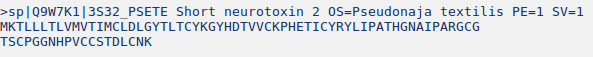
\includegraphics[width=1\linewidth, height=5cm]{./images/cadena} 
\caption{Cadenas $\alpha$ y $\beta$ de hemoglobina bovina}
\label{fig:subim3}
\end{subfigure}
 
\caption{Biomoléculas de ADN y péptidos llevadas a cadenas de strings.}
\label{fig:image2}
\end{figure}

Con respecto a estas 2 últimas estructuras, la diferencia visual más notoria radica en la cantidad de diferentes letras (strings) que las componen, para el ADN son 4 [8] y son denominadas \textbf{bases nitrogenadas} que son las siguientes:

\begin{enumerate}
\item Adenina
\item Timina
\item Citosina
\item Guanina
\end{enumerate}

Para las proteínas, su elemento básico, como ya se mencionó anteriormente es el \textbf{aminoácido}, pero ahora se adentrará en más detalle sobre esta molécula.

\subsection{Aminoácidos}

Continuar